\documentclass{article}
% \documentclass[11pt,letterpaper]{article}

% if you need to pass options to natbib, use, e.g.:
%     \PassOptionsToPackage{numbers, compress}{natbib}
% before loading neurips_2020

% ready for submission
% \usepackage{neurips_2020}

% to compile a preprint version, e.g., for submission to arXiv, add add the
% [preprint] option:
%     \usepackage[preprint]{neurips_2020}

% to compile a camera-ready version, add the [final] option, e.g.:
%     \usepackage[final]{neurips_2020}

% to avoid loading the natbib package, add option nonatbib:
\usepackage{amsmath,amssymb,latexsym,amsthm,cleveref}
\usepackage{fullpage}
\usepackage{geometry}
\usepackage{textcomp}
\usepackage{xcolor}
\usepackage{varioref}
\usepackage{bm}
\usepackage[ruled]{algorithm2e}
\geometry{margin=1in}

\usepackage[preprint]{neurips_2020}
\usepackage[nonatbib]{neurips_2020}

\usepackage[utf8]{inputenc} % allow utf-8 input
\usepackage[T1]{fontenc}    % use 8-bit T1 fonts
\usepackage{hyperref}       % hyperlinks
\usepackage{url}            % simple URL typesetting
\usepackage{booktabs}       % professional-quality tables
\usepackage{amsfonts}       % blackboard math symbols
\usepackage{nicefrac}       % compact symbols for 1/2, etc.
\usepackage{microtype}      % microtypography

\usepackage{graphicx}

\graphicspath{ {./images/} }

\title{Quantitative trading based on AlphaNet}

% The \author macro works with any number of authors. There are two commands
% used to separate the names and addresses of multiple authors: \And and \AND.
%
% Using \And between authors leaves it to LaTeX to determine where to break the
% lines. Using \AND forces a line break at that point. So, if LaTeX puts 3 of 4
% authors names on the first line, and the last on the second line, try using
% \AND instead of \And before the third author name.
%\author{%
%  \\
%  \texttt{} \\
%  \And
%   \\
%  \texttt{} \\
%}

\begin{document}

\maketitle

\begin{abstract}
  \hspace{16}In recent years, many machine learning algorithms have been successfully applied in the field of quantitative trading. However, most of them are multi-step methods, which means manual intervention is required by them. As end-to-end methods, deep learning models can overcome this shortcoming. Combined with GRU, the AlphaNet has been applied in quantitative trading and achieves good performance on some datasets. Motivated by attention based Transformer which has outperformed recurrent models like LSTM and GRU on many sequence processing tasks, we would like to replace AlphaNet's GRU with Transformer to improve model's performance on stock return prediction. Experiment results show that our model performs better than previous AlphaNet on both RMSE in return prediction and profits making in backtest. We also did analysis for history length and ablation experiments.
\end{abstract}

\section{Introduction}
\hspace{16}At present, most quantitative trading algorithms rely on high-frequency trading, which requires high hardware facilities such as network speed. The recent application of machine learning algorithms in designing automated trading systems can help reduce latency requirements by predicting stock prices in advance based on historical data.\cite{can_ml}

\hspace{16}However, many applied machine learning methods still requires manual intervention.\cite{huatai_gp} To solve this problem, some end-to-end deep learning methods have been applied in this field. For example, one of the famous computer vision models, AlphaNet \cite{alphanet}, has been modified and applied to predict the stock return. \cite{huatai_alphanet} This modified AlphaNet (we call it previous AlphaNet in the following) relies on gated recurrent unit (GRU) to process the time sequential features and performs well on some quantitative trading datasets.

\hspace{16}In the fields of natural language processing and sequential data processing, recurrent or convolutional neural networks were dominant models until Transformer was proposed.\cite{transformer} Transformer eschewed recurrent structures and solely made use of attention mechanism, achieving much better performance than traditional recurrent models on many tasks.\cite{transformer}\cite{transformer_better1}\cite{transformer_better2} Motivated by this, we would like to replace GRU in previous AlphaNet with Transformer to improve the model's ability of processing sequential features.

\hspace{16}We trained both previous AlphaNet and our model on different time periods and predicted stock return. We used root mean squared error (RMSE) as the metric and did backtest with a trading strategy as well. For long term return, our model performs better than previous AlphaNet in return prediction, and in backtest, our model also makes more profits in general. In addition, history length analysis shows that the advantage of our model over previous AlphaNet is obvious when history length is not very large. And the ablation experiments verify the effectiveness of almost every part in our model, especially Transformer. 


% We proposed our method based on the existing AlphaNet model.\cite{huatai_alphanet} Compared with traditional machine learning based models in the past, the advantage of this model is that it can predict stock return without manual intervention, automatically adjusting parameters according to market conditions, and automatically executing strategies. Such advantage can reduce information loss and improve prediction accuracy in quantitative trading. Additionally, compared with previous AlphaNet model \cite{huatai_alphanet}, our model replaces GRU with Transformer, which improves the ability of processing sequential data.

\section{Related Work}
\hspace{16}Many existing machine learning methods are being applied in the quantitative trading.\cite{decision_tree}\cite{linear} K-nearest neighbor algorithm can be used for predicting stock price in business. The predictions can be extremely close and almost parallel to the actual prices. Not only it's robust with very small ratio according to the results, but also the results are rational and reasonable.\cite{knn}
Boosting algorithm can also be applied in quantitative trading and has great performance on many datasets.\cite{boosting} However, these models require manual intervention in the training, which might lead to information loss and affect prediction accuracy.

\hspace{16}On the neural networks side, graph convolutional networks are used to capture stock market features. Combining the features extracted by the graph convolutional network with CNN, the stock market features and individual stock features are combined into joint features for stock trend prediction\cite{cnn}, which is an effective stock trend prediction method. There is also a lot of research on time series neural networks. The main content is to enable the convolution kernels in CNN to memorize long-term information\cite{tcn}. For example, the number of convolution kernels increases exponentially with the depth of the network. This type of convolutional network has been shown to perform well in extracting high-level features from structured data. However, the structure of the above models is too complex, resulting in poor performance in transfer learning or practical applications, such as running too slowly. We use the above models as inspiration to try to find a simple stock trend prediction model.


\section{Method and Approach}
\subsection{Overall model}

\hspace{16}The overall structure of our model is shown in Figure~\ref{fig:model}. For each stock, we construct a data image based on several features of it, which is the input of our model. Two feature expansion layers consisting of six functions will process the input features. The expanded features will be normalized by batch normalization layers. Since the obtained features are still time sequential features, they are processed by sequential models. In the previous AlphaNet, these features are processed by GRU. In our model, we replace GRU with two Transformer encoders to improve the model's ability of processing sequential data. Then, the processed features from two Transformers are processed by batch normalization layers. Next, the normalized features are flattened or pooled after being concatenated. Last, a fully connected layer receives the concatenated feature to predict the label.


\begin{figure}[htbp]
\centering{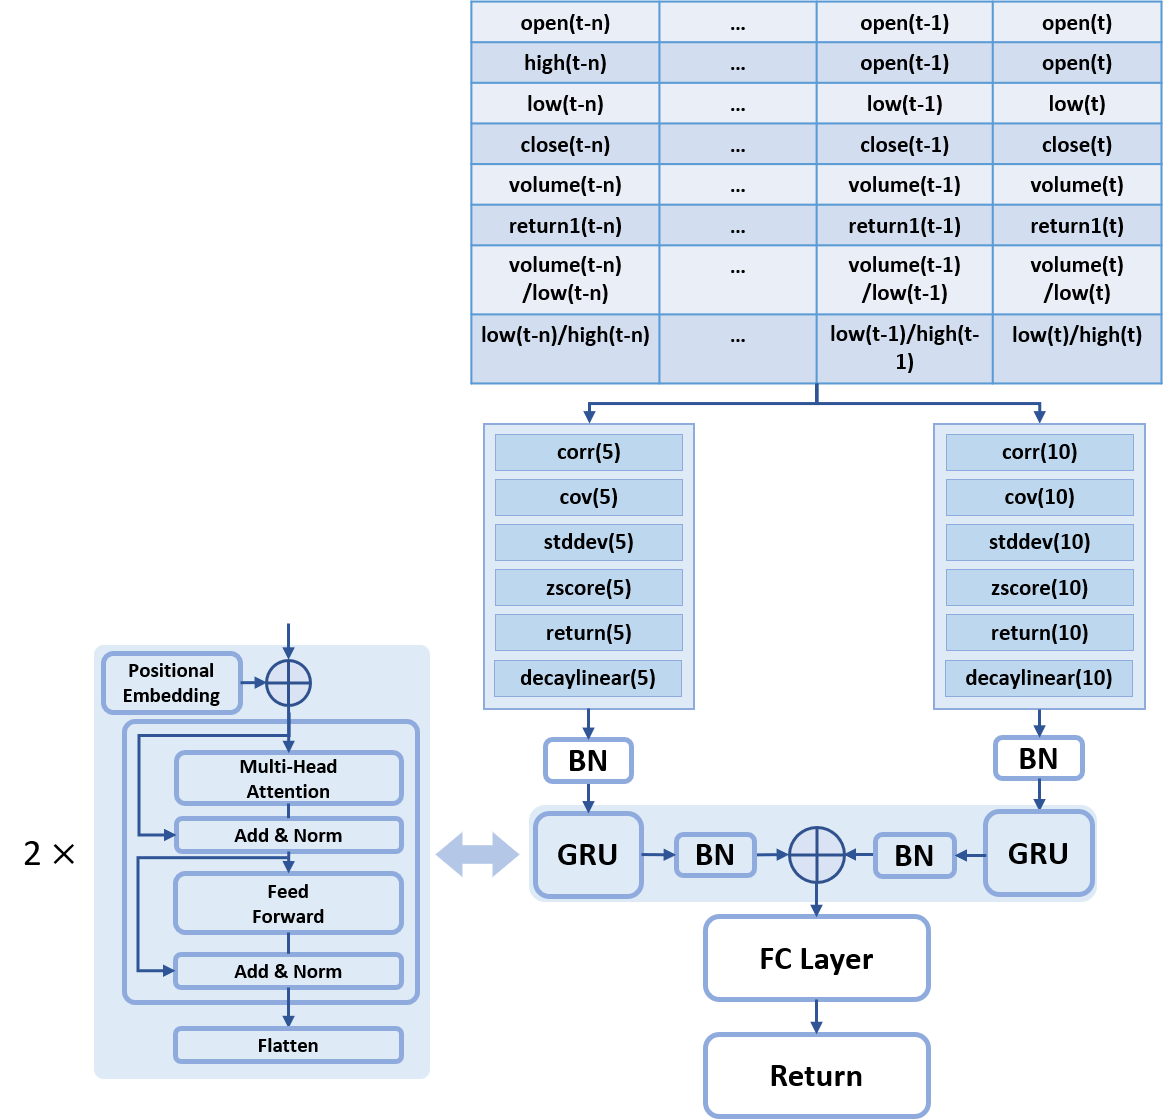
\includegraphics[width=0.6\linewidth]{images/model.png}}
    \caption{model structure}
    \label{fig:model}
\end{figure}

\subsection{Data image}
\hspace{16}The data image of each stock is shown in the top of Figure~\ref{fig:model}. In the data image, each column denotes a time step (a single day), and each row refers a different feature. There are eight features in the data image, open (opening price), high (highest price), low (lowest price), close (closing price), volume, return1 (one-day return), and two ratios volume/low and low/high.

% \begin{table}[htb]
% \centering
% \caption{Data image}
% \label{tab:data_image}
% \begin{tabular}{|c|c|c|c|}
% \hline 
% open(t-n)&...&open(t-1)&open(t)\\
% \hline  
% high(t-n)&...&high(t-1)&high(t)\\
% \hline  
% low(t-n)&...&low(t-1)&low(t)\\
% \hline  
% close(t-n)&...&close(t-1)&close(t)\\
% \hline  
% volume(t-n)&...&volume(t-1)&volume(t)\\
% \hline
% return1(t-n)&...&return1(t-1)&return1(t)\\
% \hline 
% volume(t-n)/low(t-n)&...&volume(t-1)/low(t-1)&volume(t)/low(t)\\
% \hline 
% low(t-n)/high(t-n)&...&low(t-1)/high(t-1)&low(t)/high(t)\\
% \hline
% \end{tabular}
% \end{table}



\subsection{Feature expansion operator}
% \hspace{16} In our model, there are two feature expansion layers with six functions inside each of them. The first one computes the correlation coefficient for each time series of individual stride with the output features in total number of $\frac{features * (features - 1)}{2}$. The inputs are in three dimensions of $(batch size, time steps, features)$ and the outputs are in dimensions of $(batch size, \frac{time steps}{stride}, \frac{features * (features - 1)}{2})$. Similarly, the second one computes the covariance coefficient for each time series between strides. The dimensions of both input and output are the same as the correlation feature. The third one calculates the standard deviation for each stride. The dimensions of input and output are $(batch size, time steps, features)$ and $(batch size, \frac{time steps}{stride}, features)$, respectively. The fourth one divides the mean value of each stride for each sequence by its standard deviation and regards this as a feature of zscore. The dimensions of both input and output are the same as the third one. The fifth one calculates the return rate of each stride for sequences. It always divides the last number of each stride by the first number and then minus one. The $timesteps$ also needs to be an integer times of stride numbers. The last one computes the mean value of each stride between features using the linear decay as the weights. The sizes of both input and output are the same as the third one.

\hspace{16}In our model, there are two feature expansion layers consisting of six operator functions. The definitions of these functions are shown in Table~\ref{tab:op_fun}. The stride of functions in these two layers are 5 and 10 respectively. The window length is the same as the stride. For each stock, there are 8 different features at each time step. Since corr and cov are calculated for all the pairs of features and others are calculated for a single feature, there are $2\times\binom{8}{2} + 4 \times 8 = 88$ features for each time window after expansion.

\begin{table}[htb]
  \centering\small
  \caption{Operator Functions}
  \label{tab:op_fun}
\begin{tabular}{cc}
    \toprule
    Functions & Definition \\
    \midrule
    corr(X, Y, d) & Correlation coefficients between sequential array X and Y in last d days \\
    cov(X, Y, d) & Covariance between sequential array X and Y in last d days \\
    stddev(X, d) & Standard deviation of sequential array X in last d days \\
    zscore(X, d) & Quotient of average divided by standard deviation \\ & of sequential array X in last d days \\
    return(X, d) & (X - delay(X, d))/delay(X, d) - 1, delay(X, d) is the value of X d days ago  \\
    decaylinear(X, d) & Weighted average of sequential array X in last d days, weight of last i_{th} \\
    & day is 2(d + 1 - i)/(d(d + 1)) \\
    \bottomrule
  \end{tabular}
\end{table}



\subsection{GRU}
\hspace{16}GRU is a simplified variation of LSTM. Its structure is shown in Figure~\ref{fig:gru}. GRU is a recurrent model which takes the memory of the previous step $\textbf{H}_{t-1}$ as part of the input of the current step $t$. It consists of a reset gate and an update gate. These two gates takes the current input $\textbf{X}_t$ and $\textbf{H}_{t-1}$ as input to compute $\textbf{R}_t$ and $\textbf{Z}_t$.
\begin{equation*}
    \begin{aligned}
    \textbf{R}_t = \sigma(\textbf{W}_r\cdot [\textbf{H}_{t-1}, \textbf{X}_t]) \quad\quad
    \textbf{Z}_t = \sigma(\textbf{W}_z\cdot [\textbf{H}_{t-1}, \textbf{X}_t]) \\
    \end{aligned}
\end{equation*}

\hspace{16}Then, the reset gate combines the current input with previous memory.
\begin{equation*}
    \begin{aligned}
    \Tilde{\textbf{H}}_t = \tanh (\textbf{W}\cdot [\textbf{R}_t * \textbf{H}_{t-1}, \textbf{X}_t])
    \end{aligned}
\end{equation*}

\hspace{16}Last, the update gate decides the ratio of $\Tilde{\textbf{H}}_t$ and $\textbf{H}_{t-1}$ contributing to the current output and memory $\textbf{H}_t$.
\begin{equation*}
    \begin{aligned}
    \textbf{H}_t = (1 - \textbf{Z}_t) * \textbf{H}_{t-1} + \textbf{Z}_t * \Tilde{\textbf{H}}_t
    \end{aligned}
\end{equation*}

\begin{figure}[!htb]
   \begin{minipage}{0.48\textwidth}
     \centering{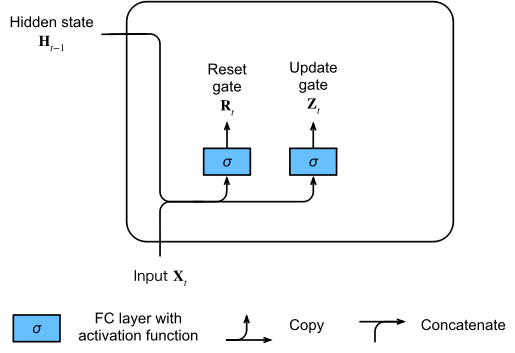
\includegraphics[width=0.8\linewidth]{images/gru.png}}
    \caption{structure of GRU}
    \label{fig:gru}
   \end{minipage}\hfill
   \begin{minipage}{0.48\textwidth}
     \centering{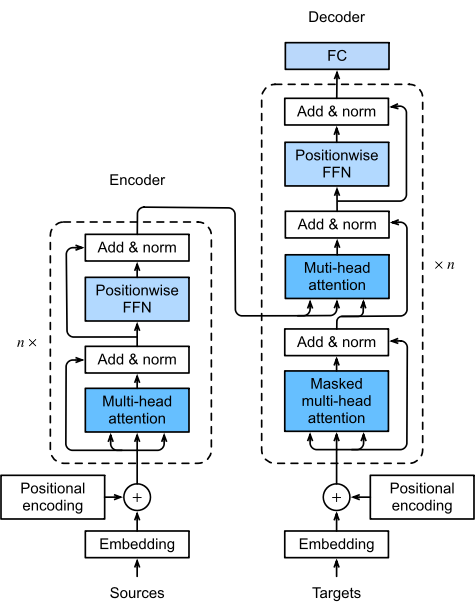
\includegraphics[width=0.8\linewidth]{images/transformer.png}}
    \caption{structure of Transformer}
    \label{fig:transformer}
   \end{minipage}
\end{figure}

% \begin{figure}[htbp]
% \centering{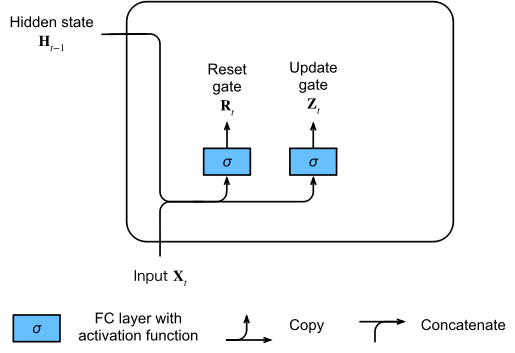
\includegraphics[width=0.4\linewidth]{images/gru.png}}
%     \caption{structure of GRU}
%     \label{fig:gru}
% \end{figure}

\subsection{Transformer}
\hspace{16}In the fields of natural language processing and sequential data processing, Transformer has good performance and performs much better than recurrent models like LSTM and GRU on many datasets, which shows Transformer's strong ability of processing sequential data.\cite{transformer}\cite{transformer_better1}\cite{transformer_better2} In our model, the expanded features obtained from feature expansion layers are still time sequential features. Therefore, we would like to replace GRU with Transformer to improve the model's performance.

\hspace{16}The structure of Transformer is shown in Figure~\ref{fig:transformer}.\cite{transformer} In the left part (encoder part) of Transformer, for input at every step, there is an embedding layer to map each input to embedding vectors. The reason for this is that in field like natural language processing, the inputs are usually words or their indices in a vocabulary list which can't be used for training directly, and embedding layer can transform these values to trainable vector features. In our model, the expanded features are trainable features already, so we don't need to do embedding for them. And our experimental results also prove that embedding is not suitable for our model.

\hspace{16}After the embedding layer, the embedding vectors are added with positional embedding vectors, since there is no recurrent units in Transformer and adding positional embedding can introduce order of sequence into the model. 

% \begin{figure}[htbp]
% \centering{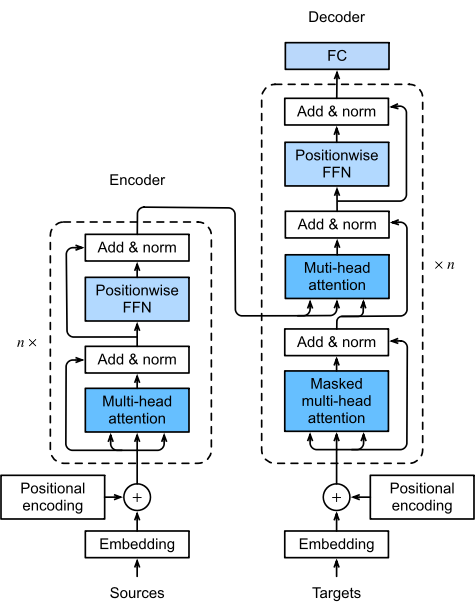
\includegraphics[width=0.4\linewidth]{images/transformer.png}}
%     \caption{structure of Transformer}
%     \label{fig:transformer}
% \end{figure}

\hspace{16}Next, the embedded features are fed into a multi-head self-attention layer. For query matrix $Q$, key matrix $K$, and value matrix $V$, the attention output is
\begin{equation*}
    \begin{aligned}
    \textrm{Attention}(Q, K, V) = \textrm{softmax}(\frac{QK^T}{\sqrt{d_k}})V
    \end{aligned}
\end{equation*}
where $d_k$ is the dimension of query and key. If $Q = K = V$, then it is self-attention. Self-attention allows every position in the input attend to all the positions. In this way, correlation between different parts of the input can be extracted and then used in the following prediction. Instead of doing a single self attention, multi-head attention is used in Transformer to attend different subspaces' information at the same time. For $Q$, $K$ and $V$, the multi-attention of them is
\begin{equation*}
    \begin{aligned}
    \textrm{MultiHead}(Q, K, V) &= \textrm{Concat}(\textrm{head}_1, \dots, \textrm{head}_h)W^O \\
    \textrm{where}\; \textrm{head}_i &= \textrm{Attention}(QW_i^Q, KW_i^K, VW_i^V)\\
    \end{aligned}
\end{equation*}
where $W^O$, $W^Q$, $W_K$ and $W_V$ are all matrices of tunable parameters.

\hspace{16}Then, after the multi-head attention layer, the obtained features are added with the input of the multi-head attention layer, and the sum features are normalized and fed into a feed-forward network which consists of two linear transformations with a ReLu activation between them.

\hspace{16}The right part (decoder part) of Transformer consists of several parts similar to those introduced above. Since we only use the encoder part of Transformer, we don't talk about the decoder in detail.

\subsection{Backtest}
\label{sec:backtest}
\hspace{16}In order to evaluate the performance of our model in the real world, a trading strategy and a backtesting framework need to be designed. We designed a simple trading strategy to test our model.

\hspace{16}Our trading strategy is to sell a stock when the forecasted return is negative, i.e. predict that the stock will fall, and buy the next time the forecasted return is positive, and vice versa. In our strategy, we hold at most one stock at a time, alternating buying and selling.


\begin{figure}[htbp]
\centering{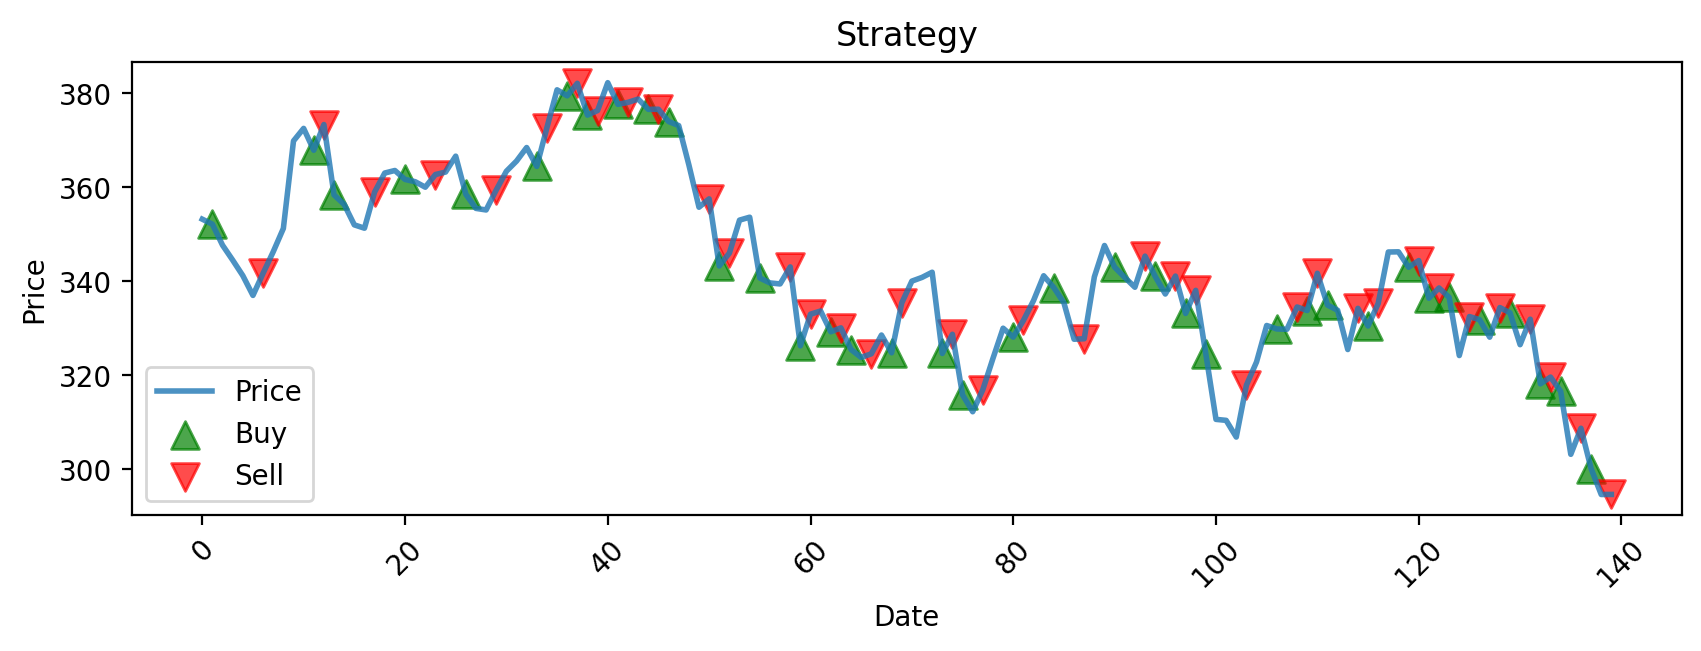
\includegraphics[width=0.8\linewidth]{images/strategy.png}}
    \caption{Example of trading strategy}
    \label{fig:strategy}
\end{figure}
\hspace{16}Figure~\ref{fig:strategy} is the trading signal chart of the strategy, and we judge the effectiveness of the model in reality through backtesting with the strategy.


\section{Experiments and Results}
\subsection{Experiments Setup}
\subsubsection{Data collection}
\hspace{16}We collect 100 stocks' daily data from Yahoo Finance. The time range is from 01/01/2015 to 10/31/2021. The data we collect includes opening price, highest price, lowest price, closing price and volume.

\subsubsection{Pre-processing}
\hspace{16}First, we use the daily closing price to compute 1-day return, 5-day return, 10-day return, 20-day return and 30-day return. For the $t_{\rm{th}}$ day, $n$-day return is
\begin{equation*}
    \textrm{Return}(t) = \frac{(p_t - p_{t-n})}{p_{t-n}}
\end{equation*}
where $p_t$ and $p_{t-n}$ is the stock price on the $t_{\rm{th}}$ and $(t-n)_{\rm{th}}$ day.
In addition, since we can't compute $n$-day return for the first $n$ days, we eliminate data on these days. Then, we calculate the ratio of volume and lowest price and the ratio of lowest price and highest price.

\subsubsection{Training details}
\hspace{16}For 5-day return, 10-day return, 20-day return and 30-day return, we use one of them as the label. For each of these labels, we construct datasets every three months from 01/31/2015. We use the data of 800 days (history length) from the beginning date as the training set, and the following 150 days as validation set, and the following 150 days as test set. We use these 9 datasets in different time periods to do the training individually, and we do the training for all the 4 labels.

\hspace{16}The hyperparameters we have tuned are shown in Table~\ref{tab:hyper_para}. For each hyperparameter, the bold value(s) is(are) optimal. "\#feature extraction layers" refers to the number of branches of feature expansion layers with different strides. "\#Transformer block layers" refers to the number of Transformer blocks stacked in each feature expansion branch. "Pooling/Flatten" refers to the operation we do to features obtained from Transformers before concatenation. We set $n$ in data image as 30, which means for each day we use the data from past 30 days to predict its label. The loss function is mean squared error (MSE). Adam is used as optimizer. Learning rate is set to 0.0001. The number of training epochs is 100. The batch size is 200.

\begin{table}[htb]
  \centering\small
  \caption{Hyperparameters}
  \label{tab:hyper_para}
\begin{tabular}{cc}
    \toprule
    hyperparameters & Values \\
    \midrule
    \#heads of the first multi-head attention layer & 1, 2, \textbf{4}, 8 \\
    \#heads of the first multi-head attention layer & 1, \textbf{2}, 4, 8 \\
    \#feature extraction layers & \textbf{2}, 3 \\
    stride of feature extraction layers & 3, \textbf{5}, \textbf{10}, 15 \\
    \#Transformer block layers & 1, \textbf{2}, 3 \\
    Pooling/Flatten & globalAverage, globalMax, \textbf{Flatten} \\
    dropout & 0, \textbf{0.1}, 0.2 \\
    \bottomrule
  \end{tabular}
\end{table}


\subsubsection{Test details}
\hspace{16}We use the trained model of each time period to do the prediction for test set in the same time period. We use root mean squared error (RMSE) to evaluate the results. The definition of RMSE is
\begin{equation*}
    \begin{aligned}
    \textrm{RMSE} = \sqrt{\frac{1}{N}\sum_{i=1}^N(y_{\textrm{pre}} -y_{\textrm{true}})^2}
    \end{aligned}
\end{equation*}
where $N$ is the number of stocks, $y_{\textrm{pre}}$ is the predicted label, $y_{\textrm{true}}$ is the true label. In addition, we do backtest for the prediction results, as mentioned in Section~\ref{sec:backtest}. We do the training and test three times for datasets at each time period and use the average results as test results.

\subsection{RMSE}
\hspace{16}For 5-day, 10-day, 20-day and 30-day return, RMSE of test sets in different time periods are shown in Figure~\ref{fig:RMSE}. We can see that for 5-day and 10-day return, our model's performance is similar to previous AlphaNet's. For 20-day and 30-day return, our model performs better than previous AlphaNet, especially for 30-day return, our model outperforms for all the beginning dates. The reason for this might be that Transformer is good at extracting very long term dependency in the input, so Transformer performs similar to GRU when the predicting label only relies on short and medium term input (i.e. 5-day and 10-day return), and the advantage of Transformer is obvious only when long term input influences the result (i.e. 20-day and 30-day return).


\begin{figure}[htbp]
\centering{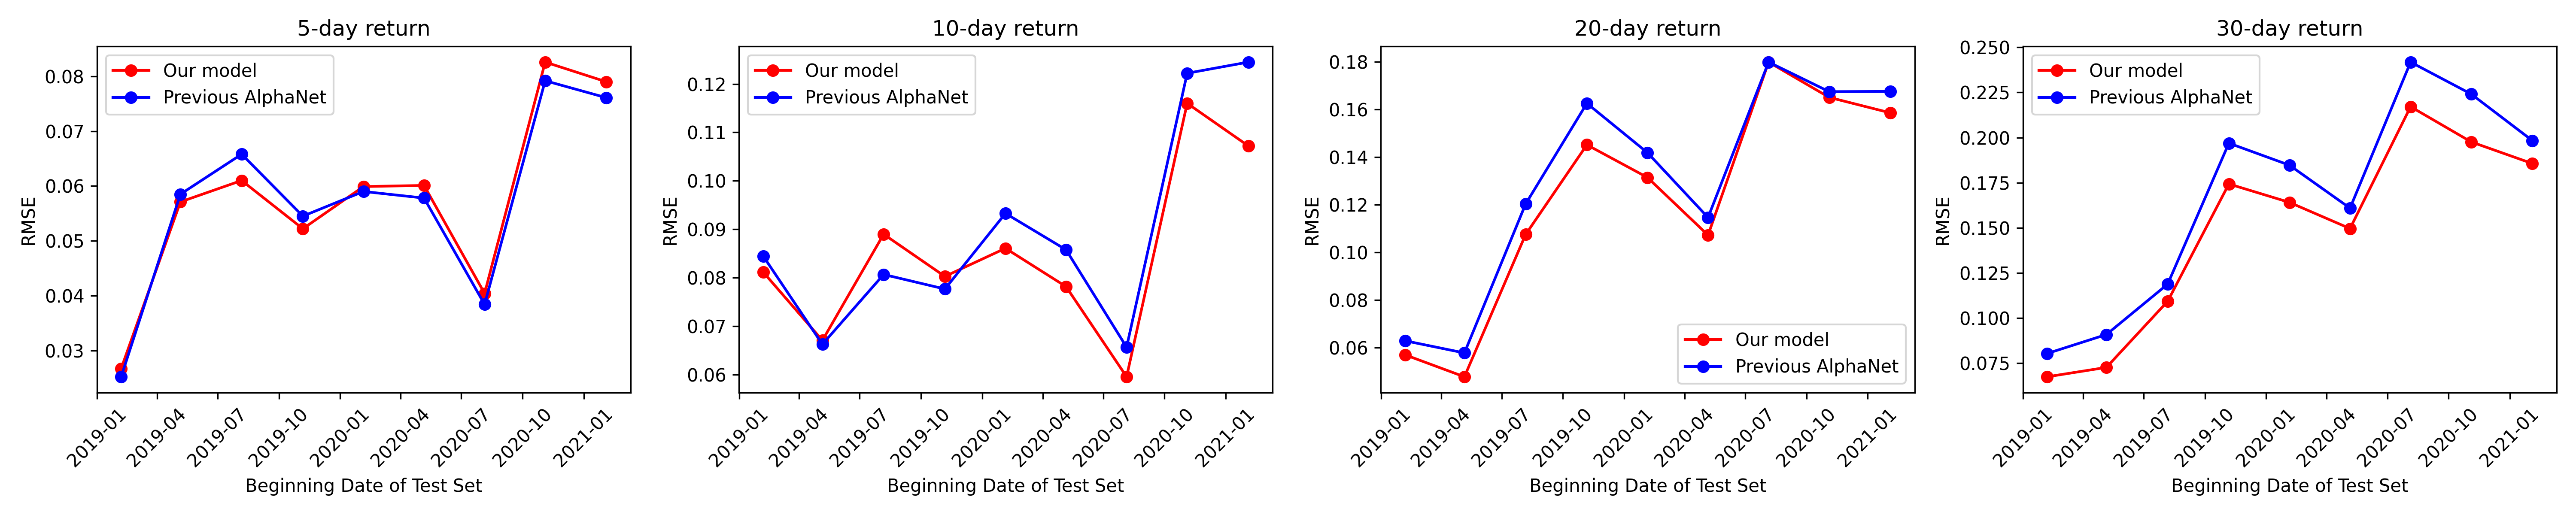
\includegraphics[width=1.0\linewidth]{images/RMSE_all_labels.png}}
    \caption{RMSE of different time periods for 5-day, 10-day, 20-day and 30-day return}
    \label{fig:RMSE}
\end{figure}

\hspace{16}The prediction and label values of 20-day return from 04/05/2019 to 11/06/2019 and 30-day return from 08/05/2020 to 03/10/2021 of stock "FB" are shown in Figure~\ref{fig:label_pre_good} and Figure~\ref{fig:label_pre_bad} respectively. The RMSE of the former is 0.0478 and 0.0578 for our model and previous AlphaNet, and the RMSE of the latter is 0.2171 and 0.2418 for our model and previous AlphaNet. We can see that smaller RMSE corresponds to better regression performance.

\begin{figure}[htbp]
\centering{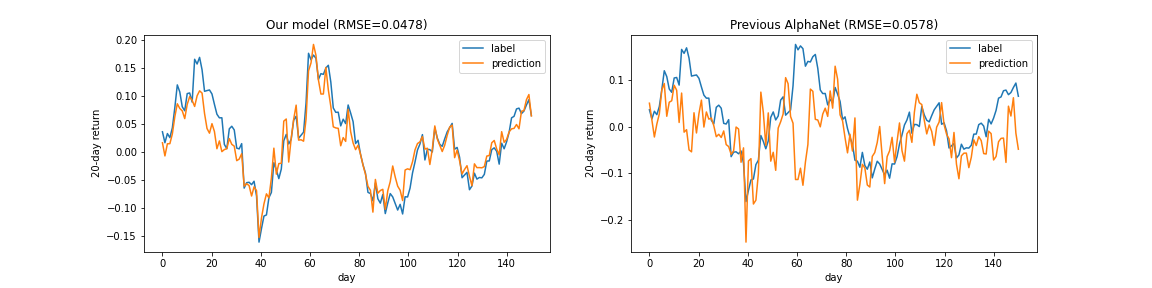
\includegraphics[width=0.8\linewidth]{images/label_pre_good.png}}
    \caption{20-day return predictions and labels from 04/05/2019 to 11/06/2019 of stock "FB"}
    \label{fig:label_pre_good}
\end{figure}

\begin{figure}[htbp]
\centering{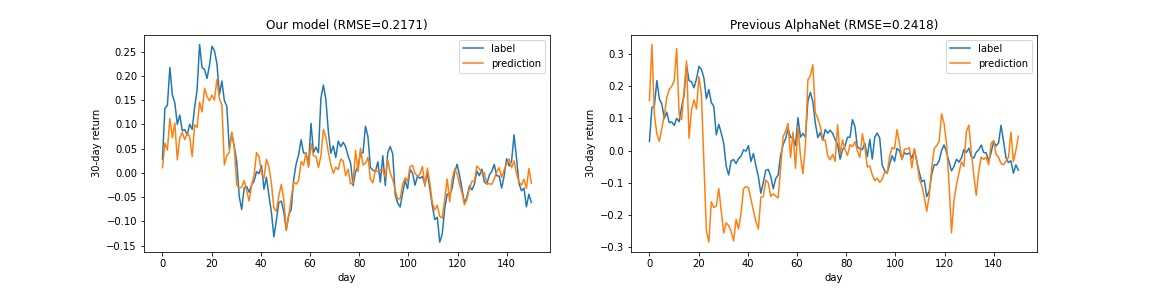
\includegraphics[width=0.8\linewidth]{images/label_pre_bad.png}}
    \caption{30-day return predictions and labels from 08/05/2020 to 03/10/2021 of stock "FB"}
    \label{fig:label_pre_bad}
\end{figure}

\subsection{Backtest}
\hspace{16}Figure~\ref{fig:btp} is the backtest results of the model, the x-axis is the test set start date, and the y-axis is the profit, in dollars per share. This profit is the average profit of all the backtested stocks. The four subfigures represent models that predict 5-day, 10-day, 20-day, and 30-day return, respectively. It can be seen that our model performs better than the previous AlaphaNet most of the time. From this we demonstrate that our model is effective in reality, and the important role of attention mechanism in processing sequential financial data.
\begin{figure}[htbp]
\centering{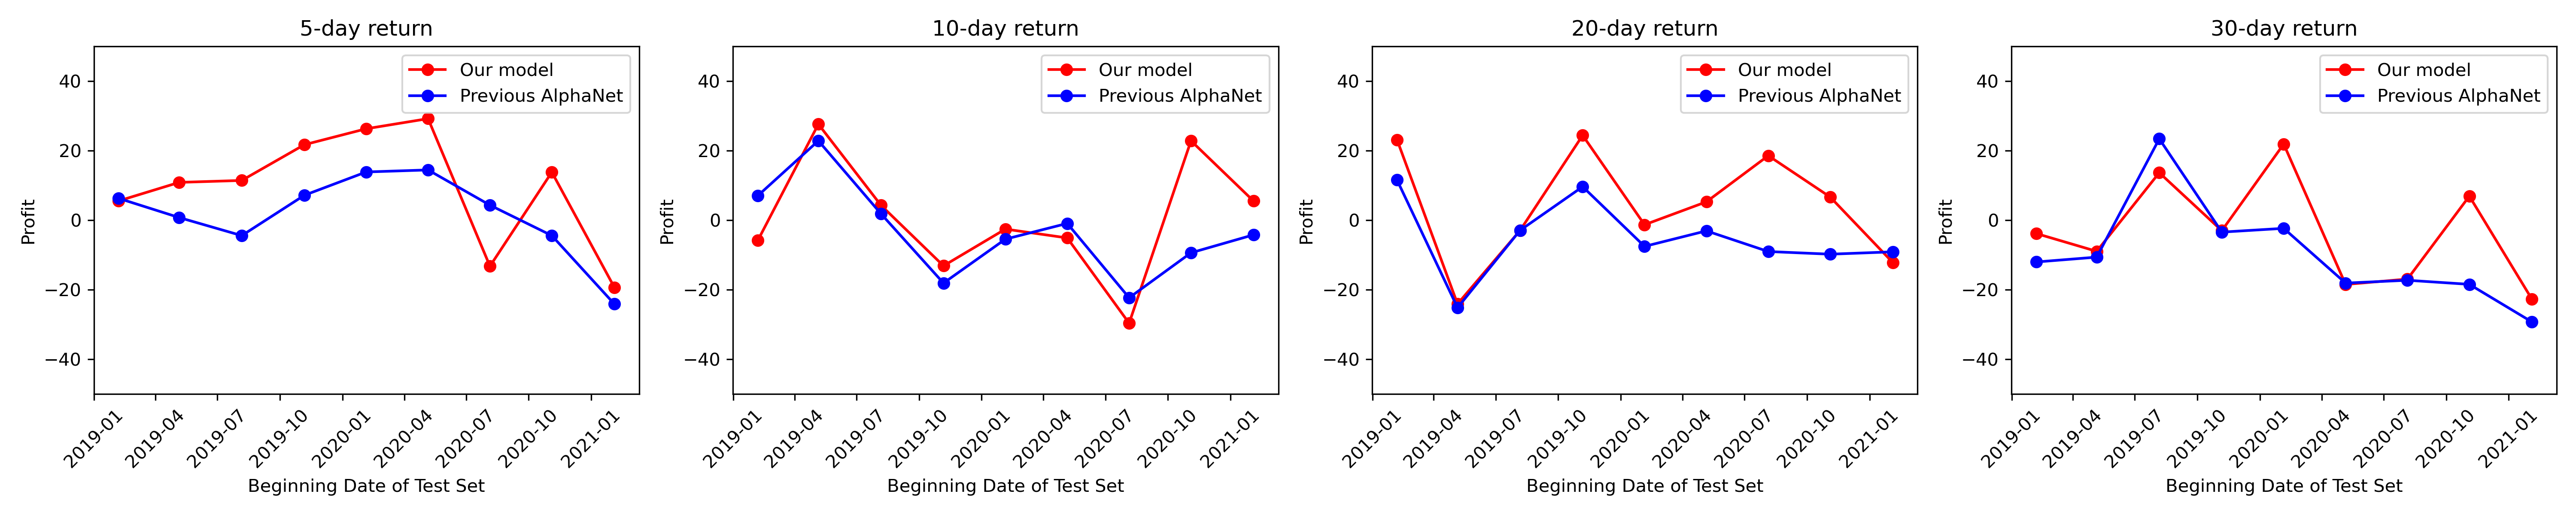
\includegraphics[width=1\linewidth]{images/s1profit.png}}
    \caption{Backtesting profit}
    \label{fig:btp}
\end{figure}
\begin{figure}[htbp]
\centering{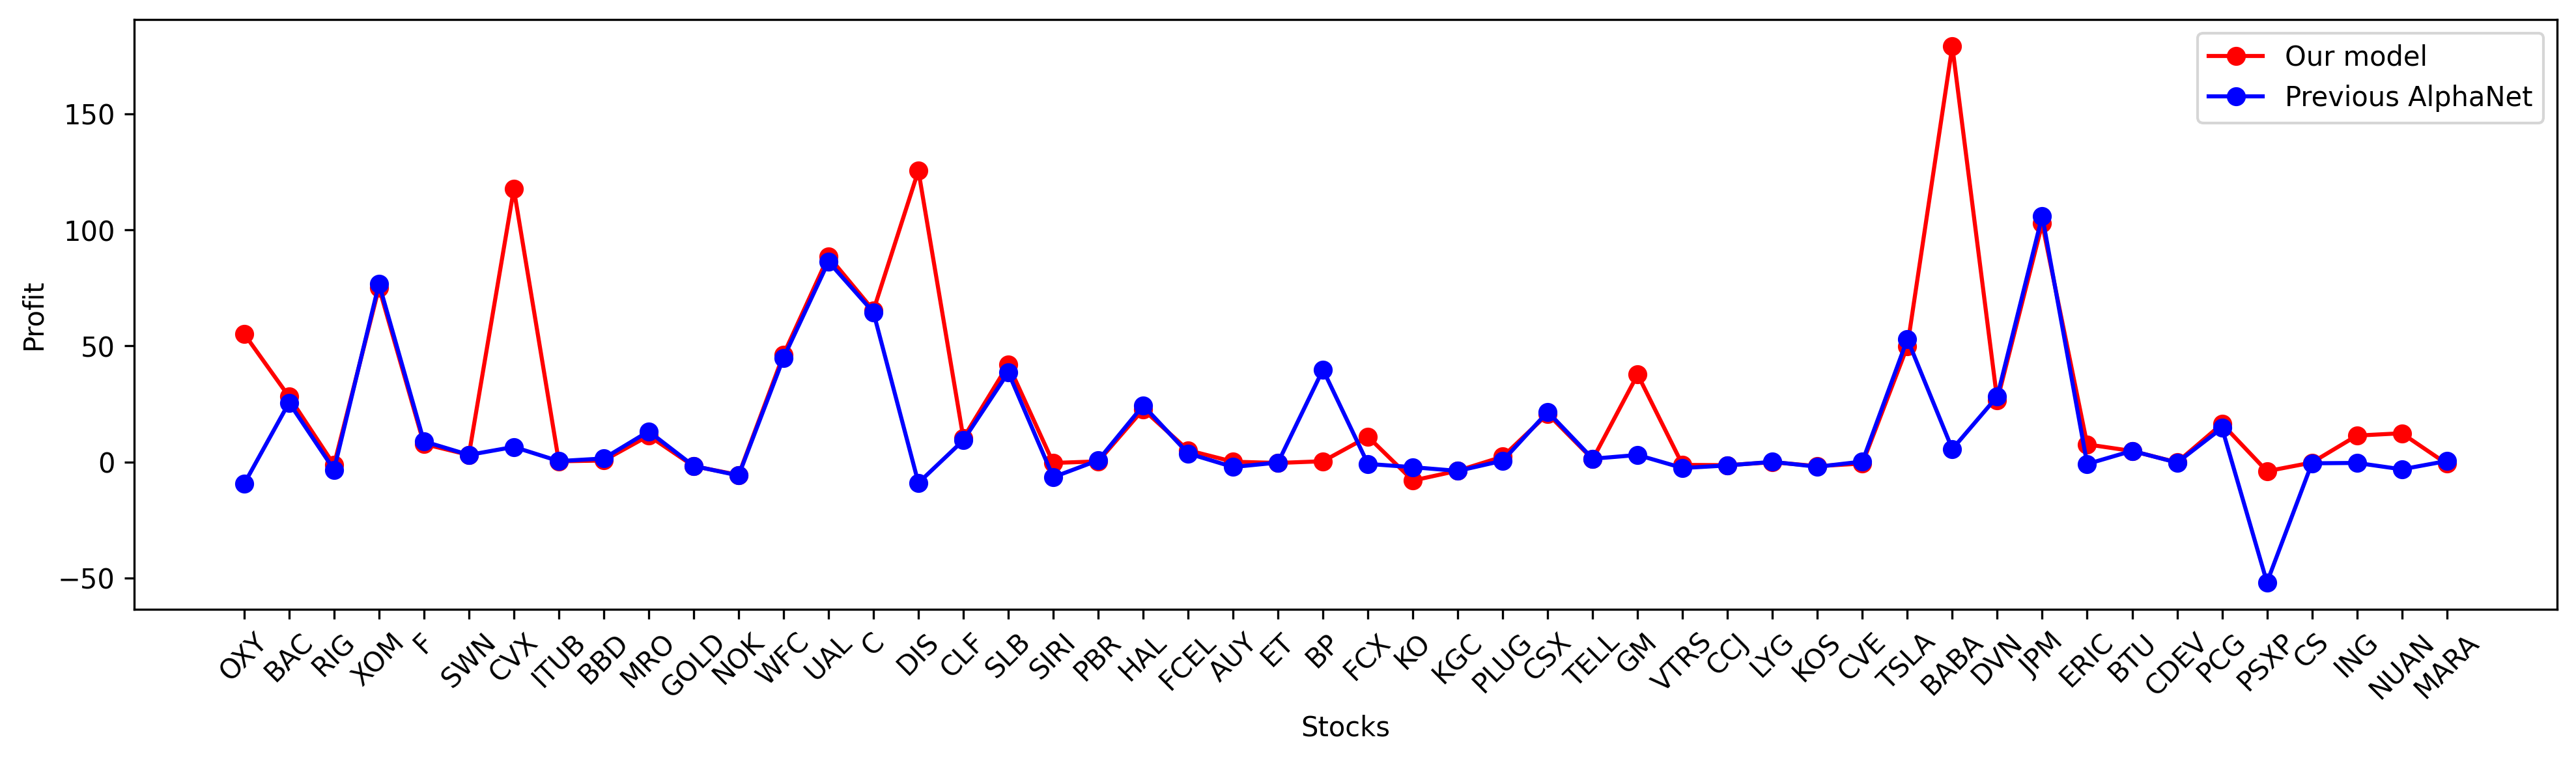
\includegraphics[width=1\linewidth]{images/diff.png}}
    \caption{All stock backtesting profit comparison }
    \label{fig:bpd}
\end{figure}

\hspace{16}Figure~\ref{fig:bpd} is an example of the profits of all listed stocks of test set from 01/07/2020 to 08/10/2020 with 20-day return as label, with stock names on the x-axis and backtested profits on the y-axis. As can be seen, our model is similar to the previous AlphaNet in most cases, but achieves much higher profits than the previous AlphaNet on some stocks.

\subsection{History Length Analysis}
\hspace{16}To analize the influence of history length, we construct datasets with history length of 400, 500, 600, 700, 800, 900, 1200, 1500 and 1800. These datasets has the same test set in the period from 08/05/2020 to 03/09/2021 with 30-day return as label, so their training set's time period are different. The results are shown in Figure~\ref{fig:history_length_analysis}.

\begin{figure}[htbp]
\centering{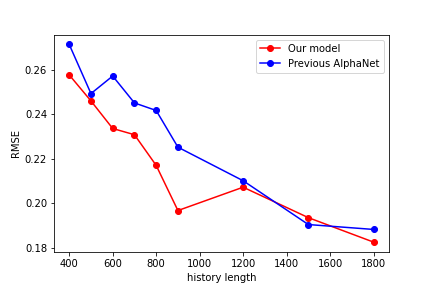
\includegraphics[width=0.4\linewidth]{images/history_length_analysis.png}}
    \caption{History length analysis}
    \label{fig:history_length_analysis}
\end{figure}

\hspace{16}As history length becomes larger, RMSE of both our model and previous AlphaNet decrease in general, because more data contributes to better performance generally. When history length is not very large, our model performs much better than previous AlphaNet. When history length is large, two model's performance becomes similar, and previous AlphaNet even outperforms our model sometimes. This shows that our model's advantage over previous AlphaNet might be obvious only when history length is not very large.

\subsection{Ablation Experiments}
\hspace{16}To analyze the contribution of each component in our model, we did ablation experiments for each part of our model. At each time, we remove one of the following components, feature expansion layer, BN1 (batch normalization layer before Transformer), Transformer, BN2 (batch normalization layer after Transformer), and we train the modified model on the dataset beginning at 04/30/2015 with history length 800 and 20-day return as label. The results are shown in Table~\ref{tab:ablation}.

\begin{table}[htb]
  \centering\small
  \caption{Ablation Experiments}
  \label{tab:ablation}
\begin{tabular}{cc}
    \toprule
    Removed component & RMSE \\
    \midrule
    None & 0.0478 \\
    Feature Expansion Layer & 0.0640 \\
    BN1 & 0.1217 \\
    Transformer & 19.1082 \\
    BN2 & 0.0483 \\
    \bottomrule
  \end{tabular}
\end{table}

\hspace{16}We can see that feature expansion layer has a little contribution to our model, while BN1 is important to the overall performance because batch normalization can help to stabilize training and shorten the time to converge. Transformer is critical to our model since we need sequential model to process the sequential expanded features. In addition, BN2 nearly contributes nothing to the performance. This might because there is a normalization layer at the end of Transformer block. Therefore, additional normalization after Transformer is unnecessary.


% When reading the source code of AlphaNet, 
% 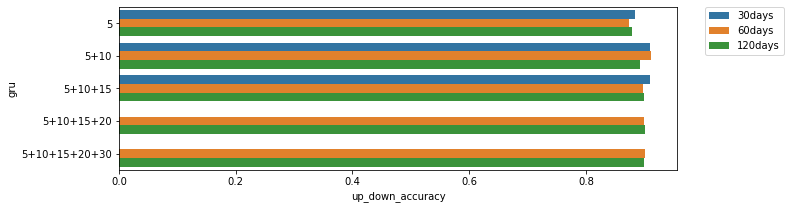
\includegraphics[scale=0.5]{gru_acc.jpg}
% 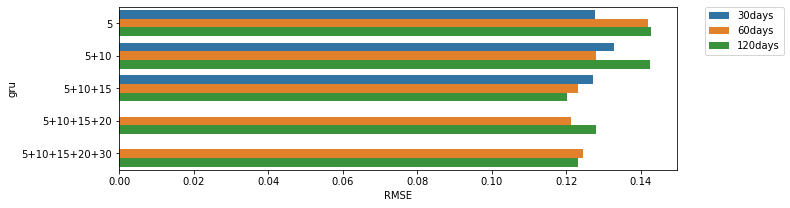
\includegraphics[scale=0.5]{gru_RMSE.jpg}


\section{Conclusions}
\hspace{16}Overall, our new model performs better than the previous AlphaNet, and the new model with the addition of the attention mechanism based Transformer achieves smaller RMSE in return prediction and more profits in backtest for multiple time periods in 2019-2021 and multiple returns of different duration. This demonstrates the effectiveness of our model and the importance of attention mechanism in financial time series data processing. In addition, history length analysis shows the advantage of our model is more obvious when history length is not too large. And the effectiveness of most components in our model is validated by the ablation experiments.

% The benefits of the model prove the effectiveness of our model, and the running speed is also much faster than the related models in the past. Thanks to the simple structure of our model, the three-month backtest running time is shortened to within ten seconds, making the Our model can be introduced into high frequency trading. In addition, we also note the importance of attention mechanism in financial time series data.



% \section{applications (put it here for now, unfinished)}
% Both transformer and GRU can be applied in explaining human behavioral data such as predicting human sentence processing. However, the transformer performs a much better fit than GRU given processing data in human languages. For the majority of training data, it shows a higher goodness-of-fit score. This is because the transformer usually pays direct attention to the single aspects at any previous positions in a sentence compared to the indirect ways of using GRU.


% \bibliography{bibfile} % put your bibtex file here
\begin{thebibliography}{}
\bibitem{can_ml} Israel, Ronen, Bryan T. Kelly, and Tobias J. Moskowitz. "Can Machines' Learn'Finance?." Journal of Investment Management (2020).
\bibitem{huatai_gp} Lin, Chen, et al. "Mining of stock selection factors based on genetic programming." Financial engineering research of Huatai Securities. 2019.
\bibitem{alphanet} Sharma, Rishab, Rahul Deora, and Anirudha Vishvakarma. "AlphaNet: An Attention Guided Deep Network for Automatic Image Matting." 2020 International Conference on Omni-layer Intelligent Systems (COINS). IEEE, 2020.
\bibitem{huatai_alphanet} Lin, Chen, et al. "AlphaNet: Factor Mining Neural Networks." Financial engineering research of Huatai Securities. 2020.
\bibitem{transformer}Vaswani, Ashish, et al. "Attention is all you need." Advances in neural information processing systems 30 (2017).
\bibitem{transformer_better1}Boogaart, E. "The GRU and Transformer explaining Human Behavioural Data represented by N400." (2019).
\bibitem{transformer_better2}Reza, Selim, et al. "A multi-head attention-based transformer model for traffic flow forecasting with a comparative analysis to recurrent neural networks." Expert Systems with Applications (2022): 117275.
\bibitem{decision_tree} Nair, Binoy B., V. P. Mohandas, and N. R. Sakthivel. "A decision tree-rough set hybrid system for stock market trend prediction." International Journal of Computer Applications 6.9 (2010): 1-6.
% \bibitem{deeplabv3} Chen, Liang-Chieh, et al. "Encoder-decoder with atrous separable convolution for semantic image segmentation." Proceedings of the European conference on computer vision (ECCV). 2018.
\bibitem{linear} Desai, V.S., Bharati, R. A comparison of linear regression and neural network methods for predicting excess returns on large stocks. Annals of Operations Research 78, 127–163 (1998).
\bibitem{knn}Alkhatib, K., Najadat, H., Hmeidi, I., & Shatnawi, M. K. A. (2013). Stock price prediction using k-nearest neighbor (kNN) algorithm. International Journal of Business, Humanities and Technology, 3(3), 32-44.
\bibitem{boosting}Rasekhschaffe, K. C., & Jones, R. C. (2019). Machine learning for stock selection. Financial Analysts Journal, 75(3), 70-88.
\bibitem{cnn}Chen, Wei, et al. "A novel graph convolutional feature based convolutional neural network for stock trend prediction." Information Sciences 556 (2021): 67-94.
\bibitem{tcn}Lea, Colin, et al. "Temporal convolutional networks: A unified approach to action segmentation." European Conference on Computer Vision. Springer, Cham, 2016.
\end{thebibliography}{}
% \bibliographystyle{abbrv}

\end{document}
